\documentclass[12pt, a4paper]{report}
\usepackage{configuration/configuration}
\usepackage{multicol}
\usepackage{multirow}
%\usepackage{nomencl}
%\makenomenclature

% Path to the Bibliography file
\addbibresource{bibliography.bib}

%\renewcommand*\nomname{List of abbrevations}

\begin{document}

% Include the frontpage, no other includes here!
\thispagestyle{empty}

\begin{center}

% Frontpage Logo

\includegraphics[width=10cm]{figures/logos/USN_logo_rgb.png}\\[5pc]

% Large title
\textbf{\Huge{Project Title}}\\[0.1pc]

% Small title
\small{CS4010: Data Management Course}\\[7pc]

% Authors of the report
\Large{Student Number}\\
\Large{Student Number}\\
\Large{Student Number}\\

% Add above for more authors. Change size to \large if it gets weird
\vfill

% The department/institution
\large{Department of Science and Industry Systems}\\[1pc]
\large{Faculty of Technology, Natural Sciences and Maritime Sciences}\\[1pc]
\large{University South-Eastern Norway, 2021}\\[1pc]

\end{center}


% Roman Page numbering and front material pages
\setcounter{page}{0}
\pagenumbering{roman}
\chapter*{Abstract}
\addcontentsline{toc}{chapter}{Abstract}
There exists a great pool of publicly available norwegian structured data on the web which can easily be fetched through API's or viewed in a HTML representation. Even though the data is readily available, creating complex searches can prove to be a challenge. Several datasources can share the same metadata such as the name of a city, country or a person with no explicit link. The semantic web creates a solution for these problems, linking the shared data together.\\

In this report we research the existing semantic web as of today, implementation methods and documents our process for transforming, linking and adding the Norwegian Public Roads Administration's parking data to the public semantic web.\\

\textbf{Keywords}: The semantic web, Norwegian parking facilities, RDF, Ontology

\chapter*{Preface}
\addcontentsline{toc}{chapter}{Preface}

For our project in the subject Data Management (CS4010) at the University of South-Eastern Norway (USN) campus Kongsberg, we have been researching the Semantic Web with the intention of publishing our own dataset to the Linked Open Data (LOD) cloud.

\vspace{5mm}


We made the decision to make our project about the Semantic Web after having gone through the materials provided on the subject “Data on the web”. Whilst studying these materials, we came across an old article about LOD in Norway \cite{semicolon_slutt}. At this point there were little doubt that this would be our project.

\vspace{5mm}

One of the first problems we faced during this project was the fact that it seems the Semantic Web is more or less dead in 2021. Most of the material we have found have been from 10 – 12 years ago. This made things more challenging than we initially anticipated. 

\vspace{5mm}

For acquiring and tranforming data, we have written software in Python, using suitable libraries to make it easy for us to produce data formatted as RDF. We also have made use of a lot of existing software like Apache Fuseki, LodView, YASGUI and Apache Airflow, for hosting and presenting the data.

\vspace{5mm}

Throughout the course of this project, we have learned a lot about semantic data and how it can be made, used, and linked. We have gotten new insight into how one goes about finding, collecting, and formatting data in accordance with the  Resource Description Framework (RDF).

\vspace{5mm}

Lastly, we are quite happy with the final result. We feel we have learned something that can be applied in the real world despite the lack of intrest in the Semantic Web. With this we mean that the individual tools and the midset we have picked up still hold value in its own right. In example can they still be used as part of a local intranet or as part of a data platform.





\chapter*{List of abbrevations}
\addcontentsline{toc}{chapter}{List of abbrevations}
%\nomenclature{RDF}{Resource Description Framework}
%\printnomenclature

\begin{itemize}
    \item[ ] LOD - Linked Open Data
    \item[ ] OWL - Web Ontology Language
    \item[ ] RDF - Resource Description Framework
    \item[ ] RDFS - Resource Description Framework Schema
    \item[ ] SPARQL - SPARQL Protocol and RDF Query Language
    \item[ ] TURTLE - Terse RDF Triple Language

\end{itemize}


\tableofcontents
\cleardoublepage

% Restart page numbering
\setcounter{page}{0}
\pagenumbering{arabic}
\clearpage

% chapters of the report
\chapter{Introduction}
Hello This is the introduction


\section{Problem Statement}
\section{Objective}

\begin{figure}[H]
  \centering
  
\includegraphics[width=0.99\linewidth]{figures/logos/USN_logo_rgb.png}
  \caption{vvvvv}
\end{figure}%
\section{Assumption and limitations}

\chapter{Theoretical Background}
%Here you write about the background information related to technologies you used.

\begin{itemize}
\item \textbf{Semantic web:} This is the web of linked data. The Semantic Web is made from web-enabled data stores, vocabularies, and rules for handling data \cite{semantic}.

\item \textbf{RDF:} Is a framework that describes resources. A resource can be anything, including documents, people, physical objects, and abstract concepts \cite{rdf}. Data that is structured in accordance with RDF, follows \textit{subject – predicate – object} triples \cite{rdf}.

\item \textbf{Ontology:} According to \cite{ontology}, an ontology is: \textit{'An ontology defines a common vocabulary for researchers who need to share information in a domain''}.

\item \textbf{TURTLE:} TURTLE is the textual representation of an RDF graph \cite{turtle}. The syntax is compact and natural and allows for an easy way to express the relationship between resources.

\item \textbf{SPARQL:} SPARQL is a query language for RDF \cite{sparql}. The syntax and semantics of SPARQL is defined by the fact that RDF is often being used for social networks, metadata, and personal information \cite{sparql}.

\item \textbf{The five stars:} We have previously mentioned that our objective includes getting a 5-star rating, but what does that mean? The five stars is a deployment scheme for LOD suggested by Tim Berners-Lee \cite{lod}. The scheme goes as follows \cite{lod}:

	\begin{enumerate}
	\item Data is published on the web in any format (png), with a license.
	\item Data is structured in a machine-readable format (xml).
	\item Data is structured in a non-proprietary format (csv).
	\item Data is structured as RDF (turtle, SPARQL).
	\item The data identifiers are linked to useful data sources.
	\end{enumerate}

\end{itemize}


\chapter{Literature Review}
%Try to do some literature review and find any similar system is existing. If yes, write how your project is different than them. If not, list similar work.\newline

Her må vi nevne at Semicolon prosjektet har jobbet med norske linkede data. 
Si at semicolon selv foreslår parkering

Og evt andre tilbydere av parkeringsdata
Si hvordan vi er bedre enn andre tilbydere av parkeringsdata, eks vegvesenet sin api. Hvordan vi forbedrer dataene og tilgjengelighet


As previously mentioned, the idea for this project came from [!]. This article was written as part of the Semicolon project \cite{semicolon}.


\section{The Semicolon project}


\section{The LOD cloud}
The linked open data cloud is a graphical representation of linked open data available on the web. Every project linked to here can be considered as similar to ours. The way our project stands out (from most of them at least) is that we have set up an automatic workflow scheduler that updates our dataset periodically. 
\chapter{Research Methodology}

\section{Choice of technology}
Even though most tools for the semantic web are written in Java, some open source libraries for Python have become availabe in recent years \cite{w3java}. Python then became an easy choice for extracting data from the sources and transforming it to LOD. For publishing the data, we chose to host a Sparql Endpoint using Apache Fuseki and use LodView to dynamically generate an HTML representation of the dataset based on the Sparql endpoint. A major benefit of this, is that Fuseki also provide access to a reasoner, ensuring that the published data is as rich as possible. Fuseki and LodView are deployed using Apache Tomcat, along with a reverse proxy in Apache HTTP server in order to make them publicy available on the internet. For representing the data as a graph we have utilized Lod Cloud Draw and \textbf{XXXXXXXXXXXXXXXXXXXX.js}

\vspace{5mm}

Although Apache Fuseki does function as a public SPARQL endpoint, security issues led us to want to hide this interface, and rather provide a separate public endpoint using YASGUI, which also gives a some extra functionality like map plotting of the query results.

\vspace{5mm}

For handling the automatic workflow scheduling, we opted for Apache Airflow as we had learned about this in class.

\vspace{5mm}

The technology choice we struggled the most with, was for the HTML representation. Here we experimented with several frameworks like Pubby and Loddy before landing on LodView, which provided all the functionality we wanted.

\section{Data collection process}
Statens vegvesen (Norwegian Public Roads Administration) \cite{statensvegvesen} provides an API for their parking data in JSON format. As the API only gives access to subsets of the data, we have created a program that fetches the complete dataset and creates a single JSON file.

\vspace{5mm}

This data is fed to a program that combines our RDF schema as seen in Appendix \ref{Appendix:ontology} and the parking data, generating RDF triples in a RDF/XML file format. The program additionally uses data from the Norwegian postal and logistics company Bring \cite{bring} to match postal codes from Statens vegvesen's data with Norwegian municipality codes. These codes are then linked with Wikidata \cite{wikidata} using their Sparql endpoint.

\vspace{5mm}

In our RDF schema, we inherit and reuse vocabularies we have found in the ontologies provided at Schema-org \cite{schema-org} and MobiVoc \cite{schema-mobivoc}.


\section{System architecture}

\begin{figure}[H]
	\centering
	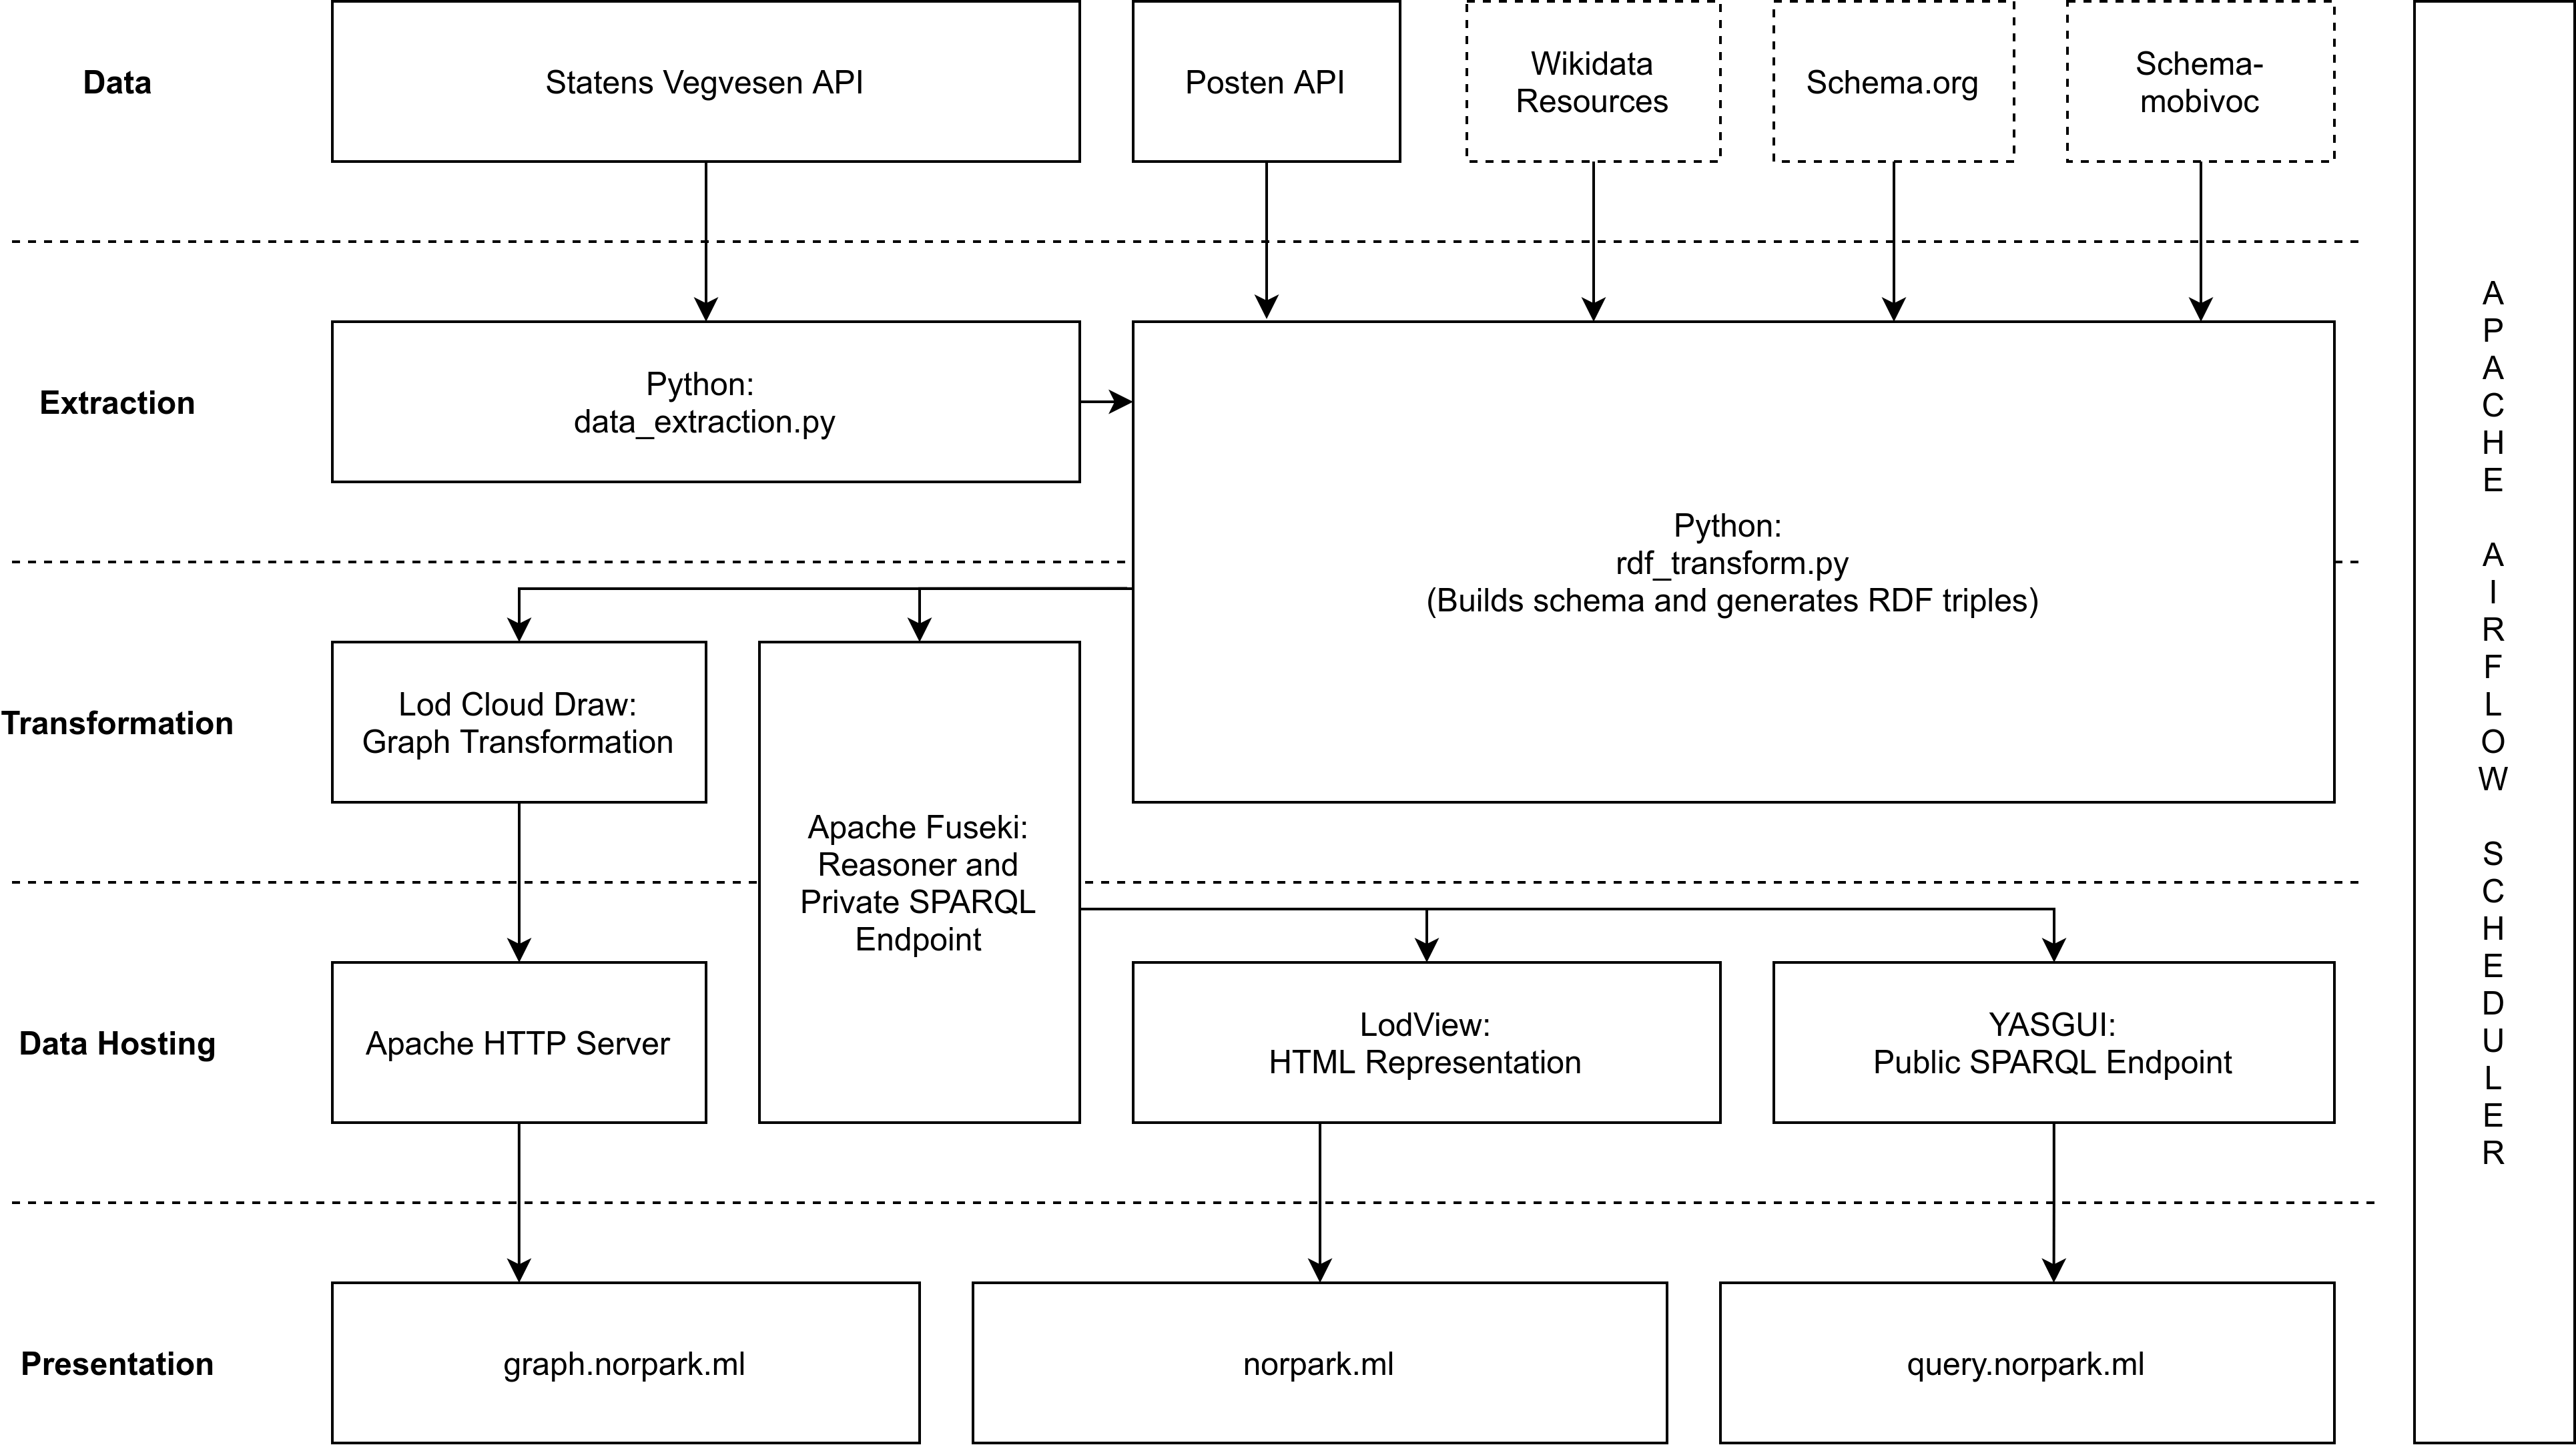
\includegraphics[width=\linewidth]{figures/system-architecture.png}
	\caption{The system architecture}
\end{figure}




\chapter{Results}
We have managed to extract, transform and publish The Norwegian Public Roads Administration's publicly available parking data to the Semantic Web. In numbers, this results in 280 892 RDF triples as seen in Appendix \ref{appendix:triples}. This makes it possible to create advanced queries to find parking facilities, that can for instance take a geographical location, numbers of handicap places and electrical vehicle chargers into account. We have linked the dataset to geographical locations in Wikidata, resulting in a total of 31 938 links to nodes outside our dataset. Great emphasis has also been put into reusing existing vocabularies, which increases the integration of our dataset with the existing Semantic Web. The integration with Wikidata also means that the number of possible queries and use cases are infinite.

\vspace{5mm}
The data is accessable through a user-friendly web interface at \url{http://norpark.ml}, where one can click through all of the parking facilites and parking companies' linked attributes and even end up on another webpage such as Wikidata.org. A screenshot of the webpage is shown in Appendix \ref{appendix:webpage}. The web interface provides an interactive map for each parking facility, making it easy to locate the facilites.

\vspace{5mm}

As mentioned, we have also provided a public SPARQL endpoint, which is accessible at \url{http://query.norpark.ml}. Here the user can execute queries on our dataset, either directly or programatically. An example of this can be seen in Appendix \ref{appendix:query}.

\vspace{5mm}

To ensure that the data that we present is always up-to-date, we have added an automatic workflow scheduler that will ensure that the data is updated periodically. A diagram of the workflow is described in Appendix \ref{appendix:airflow}.

\vspace{5mm}

As mentioned one of our goals was to publish our data on the LOD Cloud \cite{lod-cloud}, and receive a five star rating. Unfortutely they only update their graph once or twice a year, so for now, in order to see our dataset in the cloud we have generated this ourselves using their open source software. This interactive graph is made public at \url{http://graph.norpark.ml}, and a screenshot can be seen in Appendix \ref{appendix:cloud}. Our dataset colored blue and located in the top center of the cloud.

\vspace{5mm}

We are happy to say that our dataset meets all the requirements of a five star rating. 
However, as the LOD Cloud only checks the status of the dataset periodically we are currently only rated at three stars until the next update of the Cloud. This can be seen in the page of our published dataset at \url{https://lod-cloud.net/dataset/norpark} and in Appendix \ref{appendix:lod-norpark}.

%Towards the end of the project, we thought it would be nice if we could provide the people reading our dataset with a map view of some kind, so that they have a visual representation in addition to the street address and postal code. If possible, we would like to have satellite imagery, but regular maps would also work fine. We would also like it if the reader were able to move the map view around to see the surrounding area.

%To achieve this, we investigated various Python libraries, scripts, and tools that we might be able to use. Eventually when we found LodView, we were able to get not only a nicer layout, but also a map view via a JavaScript API to the openstreetmaps service. This allowed us to include a map with a pin at the top of each parking place’s page.

\chapter{Discussion and Conclusions}
%Discuss your results, challenges and conclude your work here.

The reason for initially choosing to work with LOD was because we were intrigued by the possibilities the Semantic Web provide and wanted to contribute to its evolution. However, critics of the Semantic Web claim that it is an impossible dream, and over the past few years it has lost a lot of its momentum. As it is rarely used in the industry, the existing software and frameworks are often not very mature and in many cases deprated. They also often provide lacking or overly complex documentation. The prevalent use of Java has also been a challenge as none of the group members have any previous experience with it. 

\vspace{5mm}

The duration of the project spanned three weeks. During the first week, we sat together and researched technologies, solutions and the Semantic Web while also creating small proof-of-concept programs and a baseline. The following days we split the working tasks equally among all group members and began implementing our solution.

\vspace{5mm}

As we had no background knowledge on the Semantic Web and LOD we spent a lot of time researching the subject. This further increased our time constraints for the implementation of our system. Becuase of this, and to not reinvent the wheel, we have only written our own software when necessary or sensible, and rather tried to use existing implementations like Apache Fuseki and LodView. However, they are not meant for deployment out of the box. They require a lot of configuration, and this was a major challenge and time drain within the project.

\vspace{5mm}

Our ontology and RDF schema took a lot of time in research and design, as well as finding a data source that could be linked to existing LOD. With more time, it would probably also be possible to link our data to more datasets, further integrating the Semantic Web. At first we implemented the entirety of our ontology as a separate OWL file with a completely novel vocabulary. However, according to \cite{w3-best-practices}, it is best practice to reuse existing standardized vocabularies as much as possible. Bacause we were able to do this to a large degree, we found it sufficient to integrate the novel part of our vocabulary with the individuals of our data in a single RDF file.

\vspace{5mm}

One of the major benefits of our system is our SPARQL endpoint. However, even though we have made it facilitated for complex SPARQL queries, they are still hard to write. With more time, we would have liked to explore the idea of an easy-to-use application that utilised our SPARQL endpoint. This would ensure that also non-programmers would be able to search for parking facilities.

\vspace{5mm}

There are several challenges with publishing LOD. According to \cite{can-i-sparql-your-endpoint}, SPARQL endpoints can be so resource intensive and expensive to host, that people struggle to keep their endpoints up. Were our endpoint to experience any non-trivial amount of traffic, it would require a lot of expences on our part. Another challenge is that when publishing linked data, you are entering a social contract with the Semantic Web. The IRIs of the published resources should ideally be valid forever. The namespace of our dataset relies on a free domain (norpark.ml), which we own for the next year. Are we to ensure a long life for our dataset, this too will cost money in the long run. Becuase of this, we will contact The Norwegian Public Roads Administration, and inform them about how we have improved the usability of their data. Even though private corporations does not see the benefit of publishing their data as LOD, governmental institutions should act with more altruism. Hopefully our project can serve as a springboard or inspiration for further ventures into the Semantic Web within The Norwegian Public Roads Administration.



% Bibliography
\chapter*{References}
\addcontentsline{toc}{chapter}{References}
\chead{REFERENCES}
\printbibliography[heading=none]

\chapter*{Appendices}
\appendix

\chapter{Example of a parking facility on the webpage}
\label{appendix:webpage}
\begin{figure}[H]
	\centering
	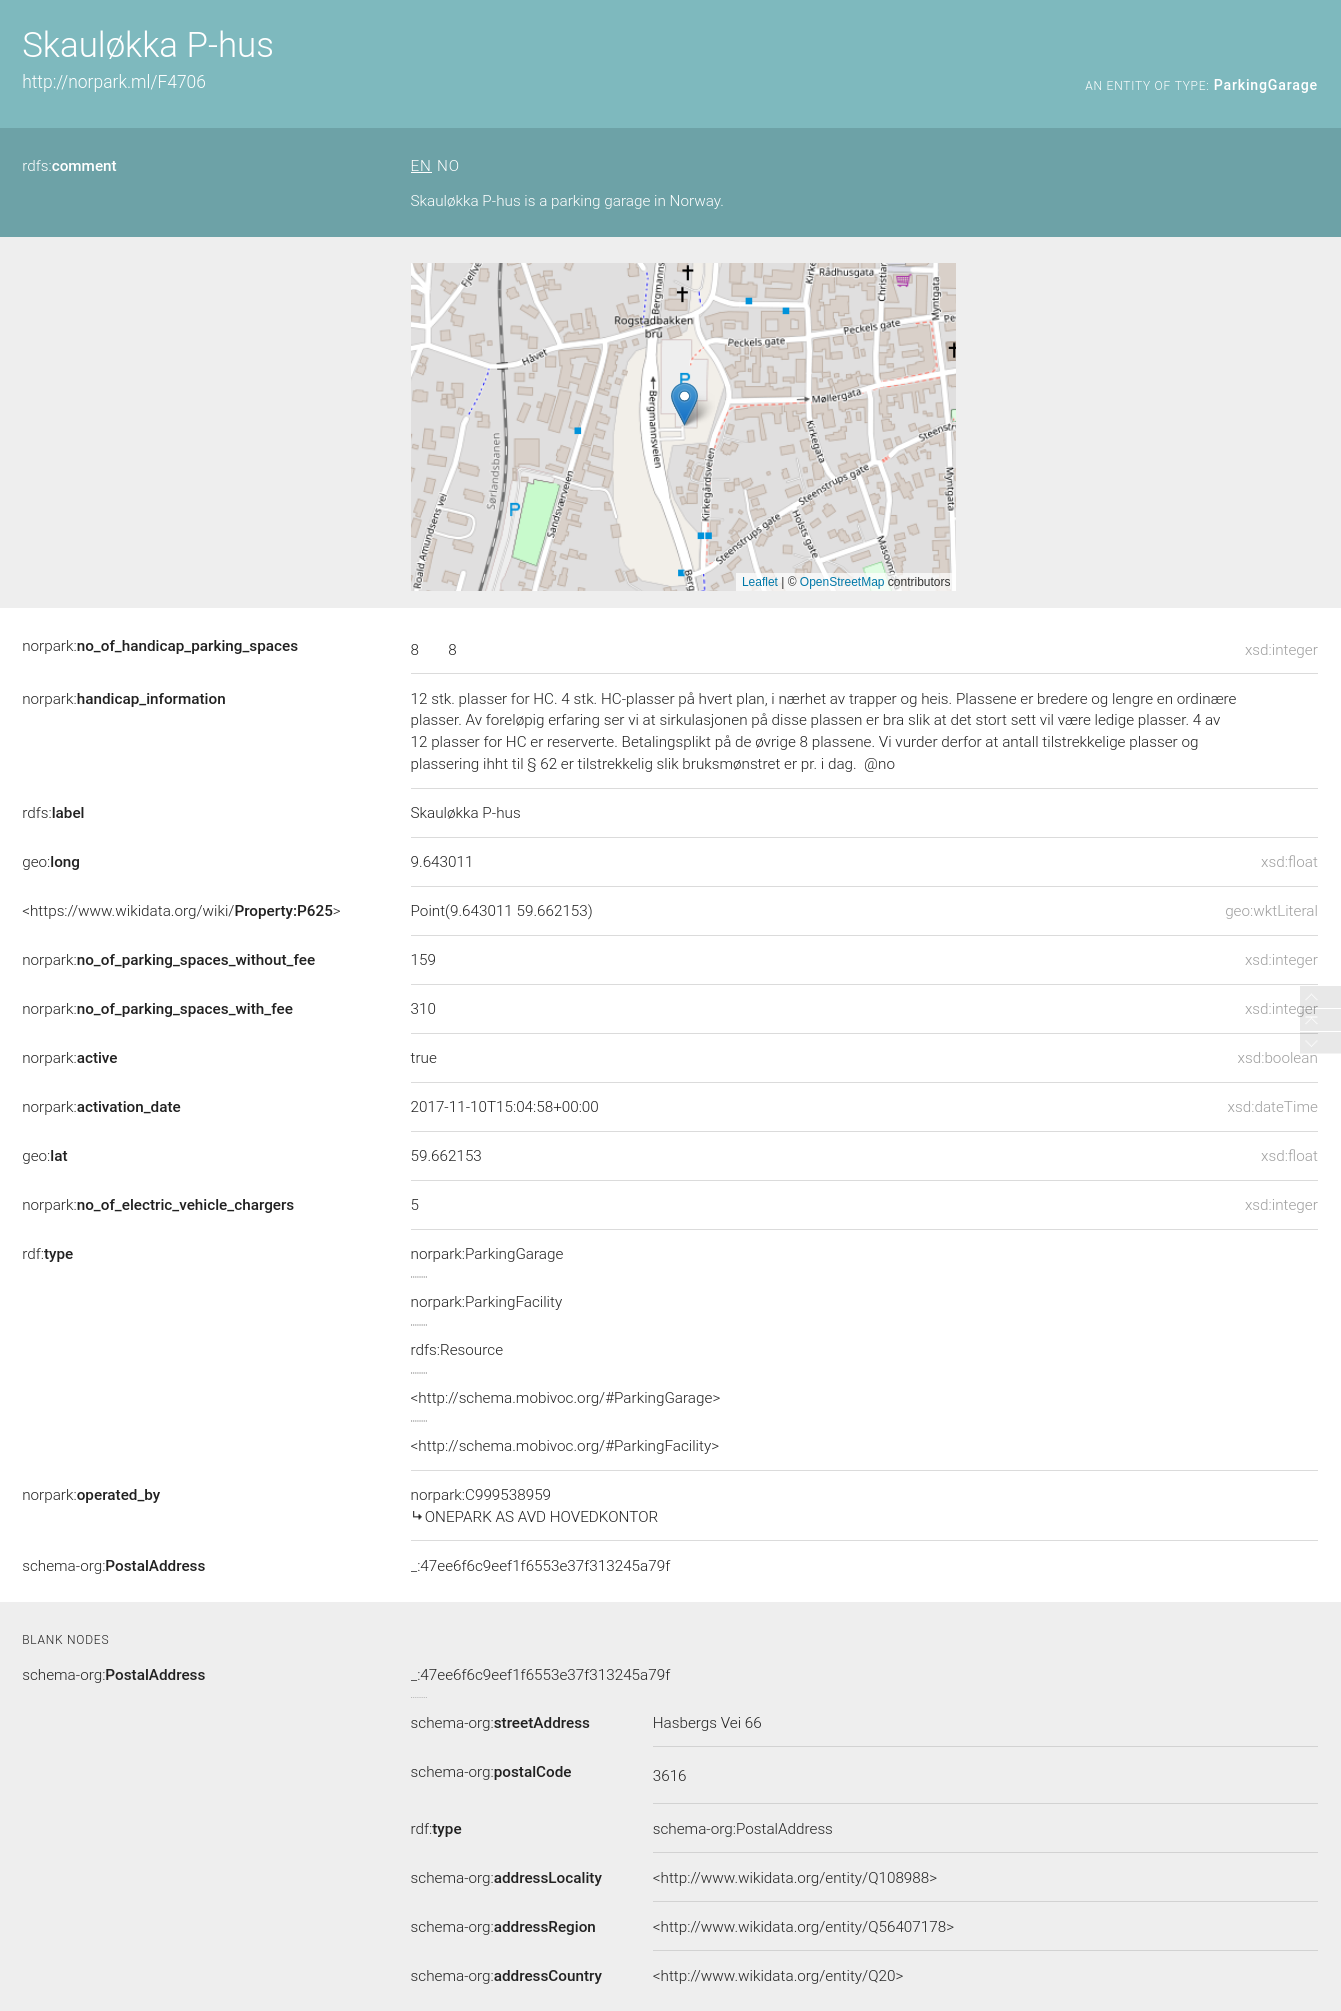
\includegraphics[scale=0.20]{figures/parking-place-screenshot.png}
	\caption{A screenshot from our webpage describing information of Kongsberg VGS' parking facility.}
\end{figure}

\chapter{Example of a query on the webpage}
\label{appendix:query}
\begin{figure}[H]
	\centering
	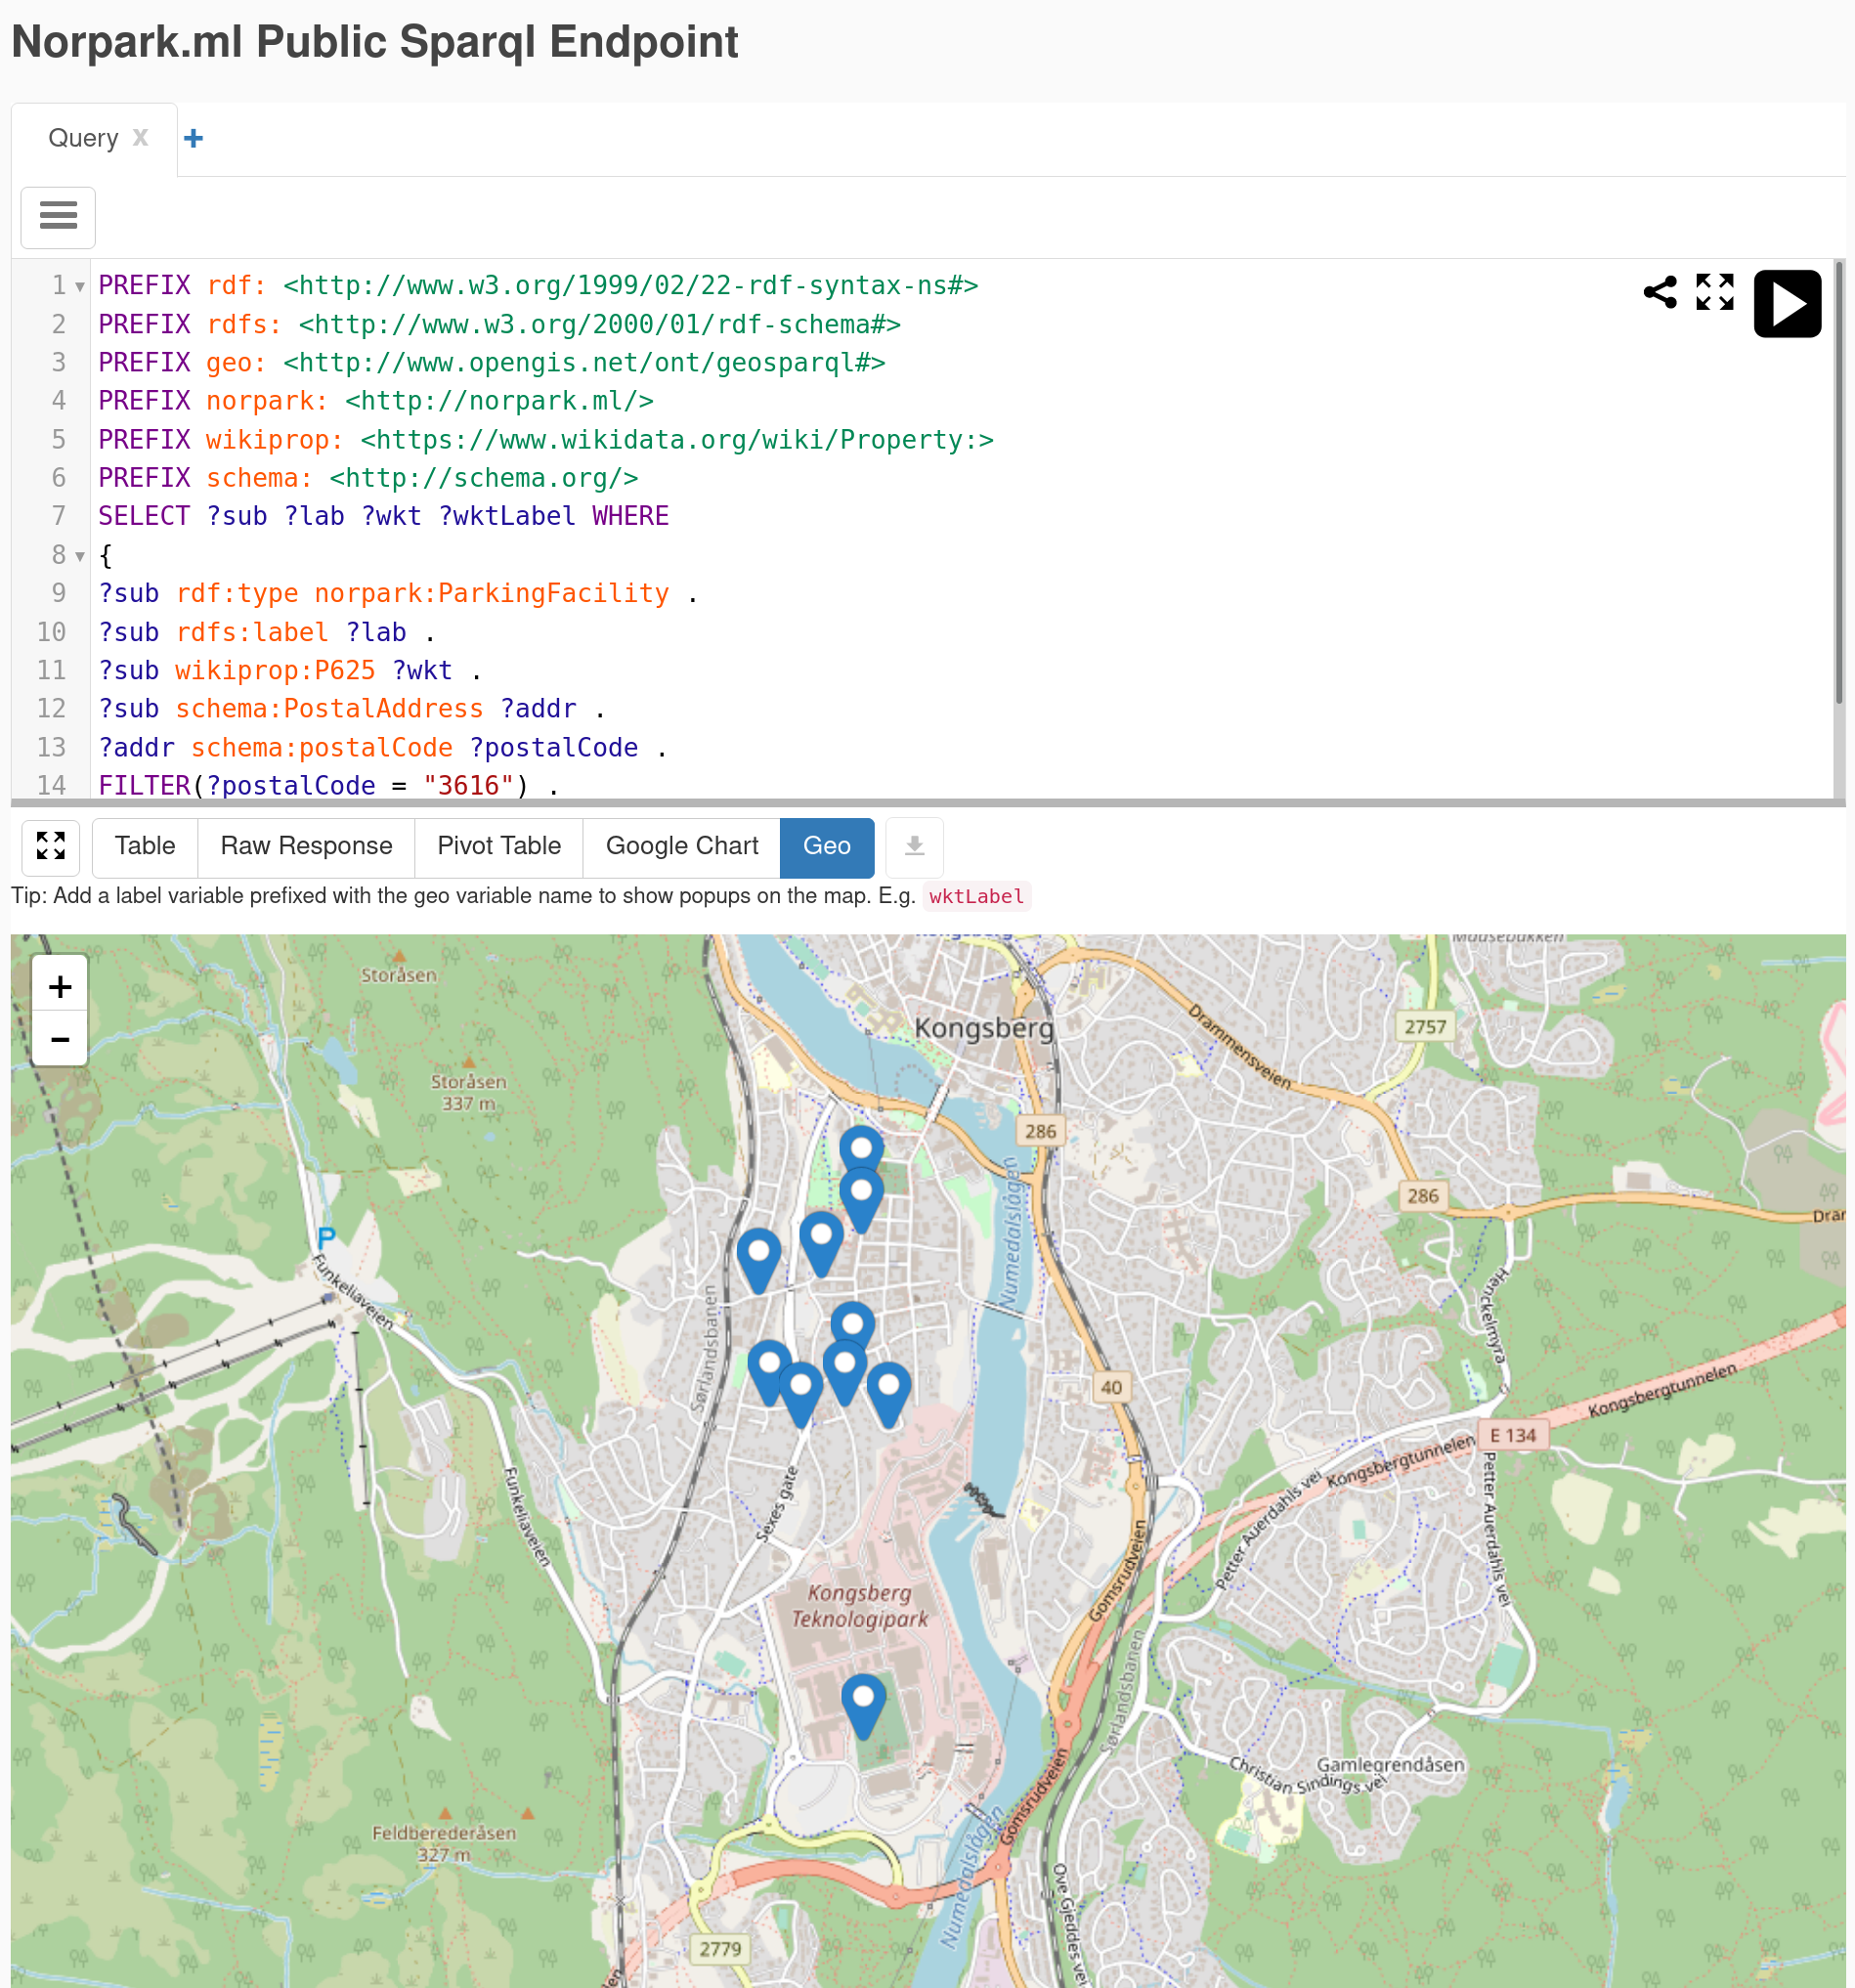
\includegraphics[width=\linewidth]{figures/query-screenshot.png}
	\caption{A screenshot from our webpage showcasing a query, resulting in a map of 10 parking facilities in Kongsberg}
\end{figure}

\chapter{LOD Cloud}
\label{appendix:cloud}
\begin{figure}[H]
	\centering
	% 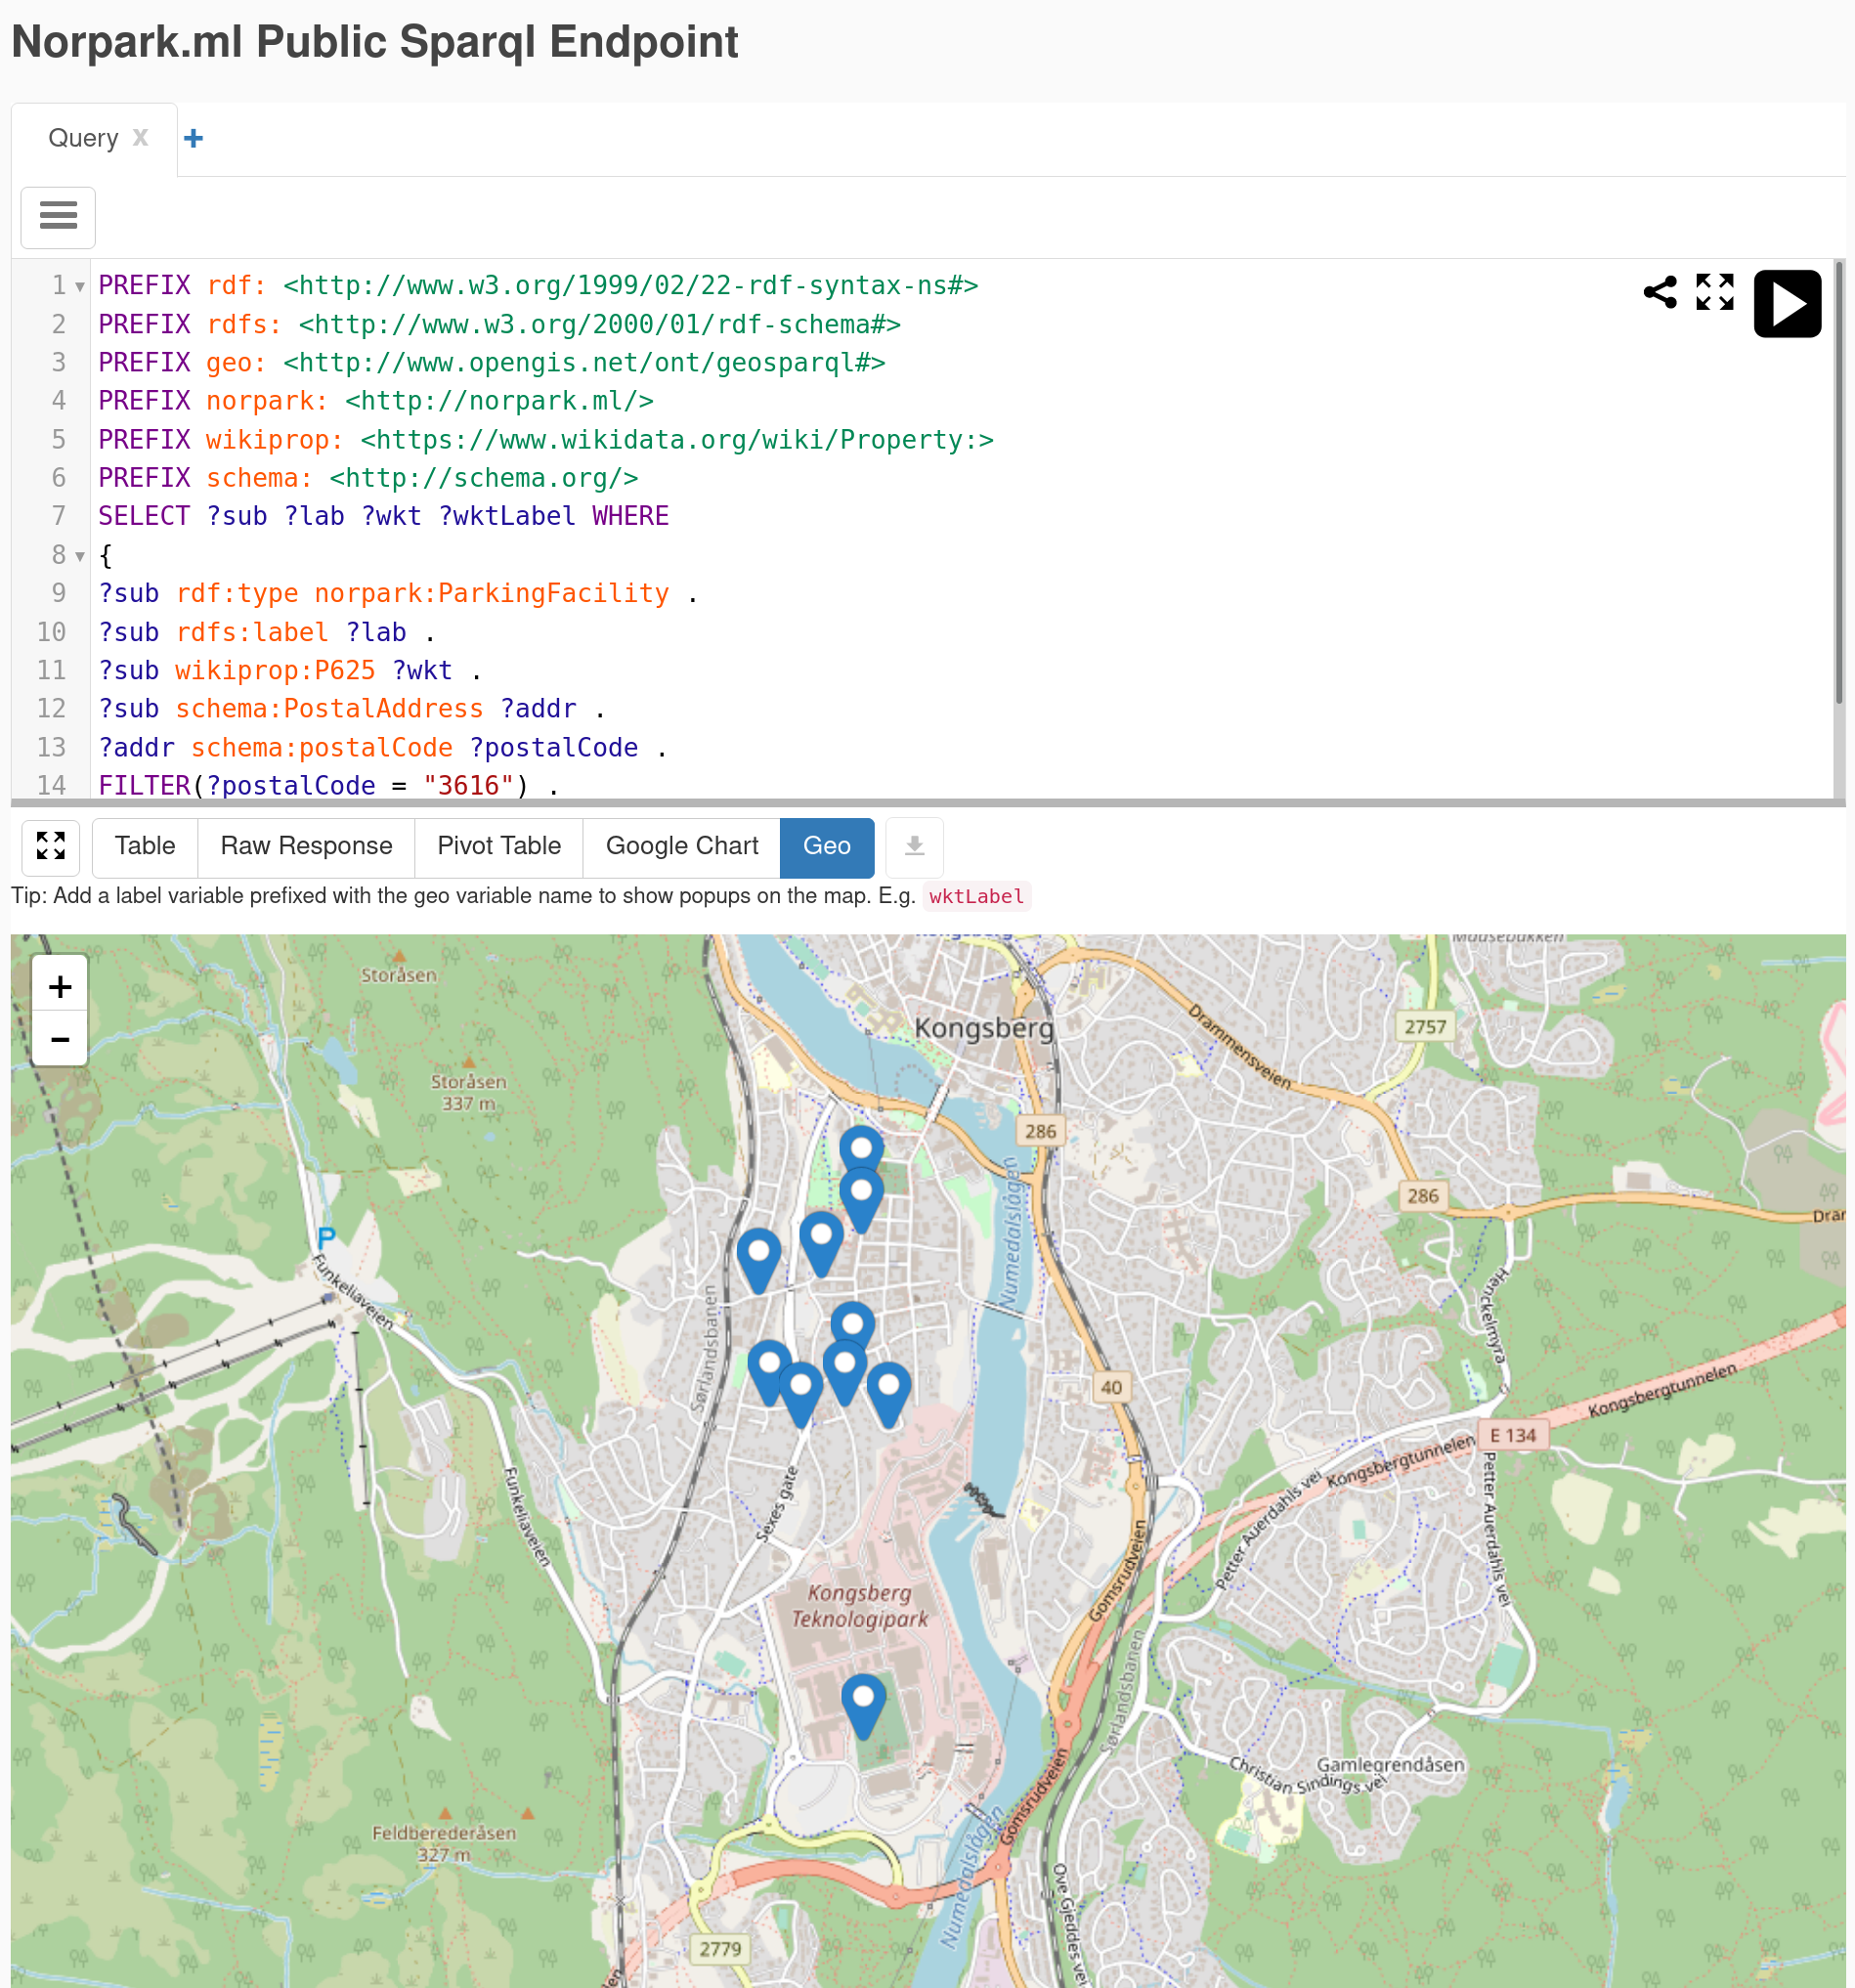
\includegraphics[width=\linewidth]{figures/query-screenshot.png}
	\caption{A screenshot of the LOD Cloud graph we generated highlighting the inclusion of our dataset. }
\end{figure}

\chapter{Norpark Dataset at LOD Cloud}
\label{appendix:lod-norpark}
\begin{figure}[H]
	\centering
	% 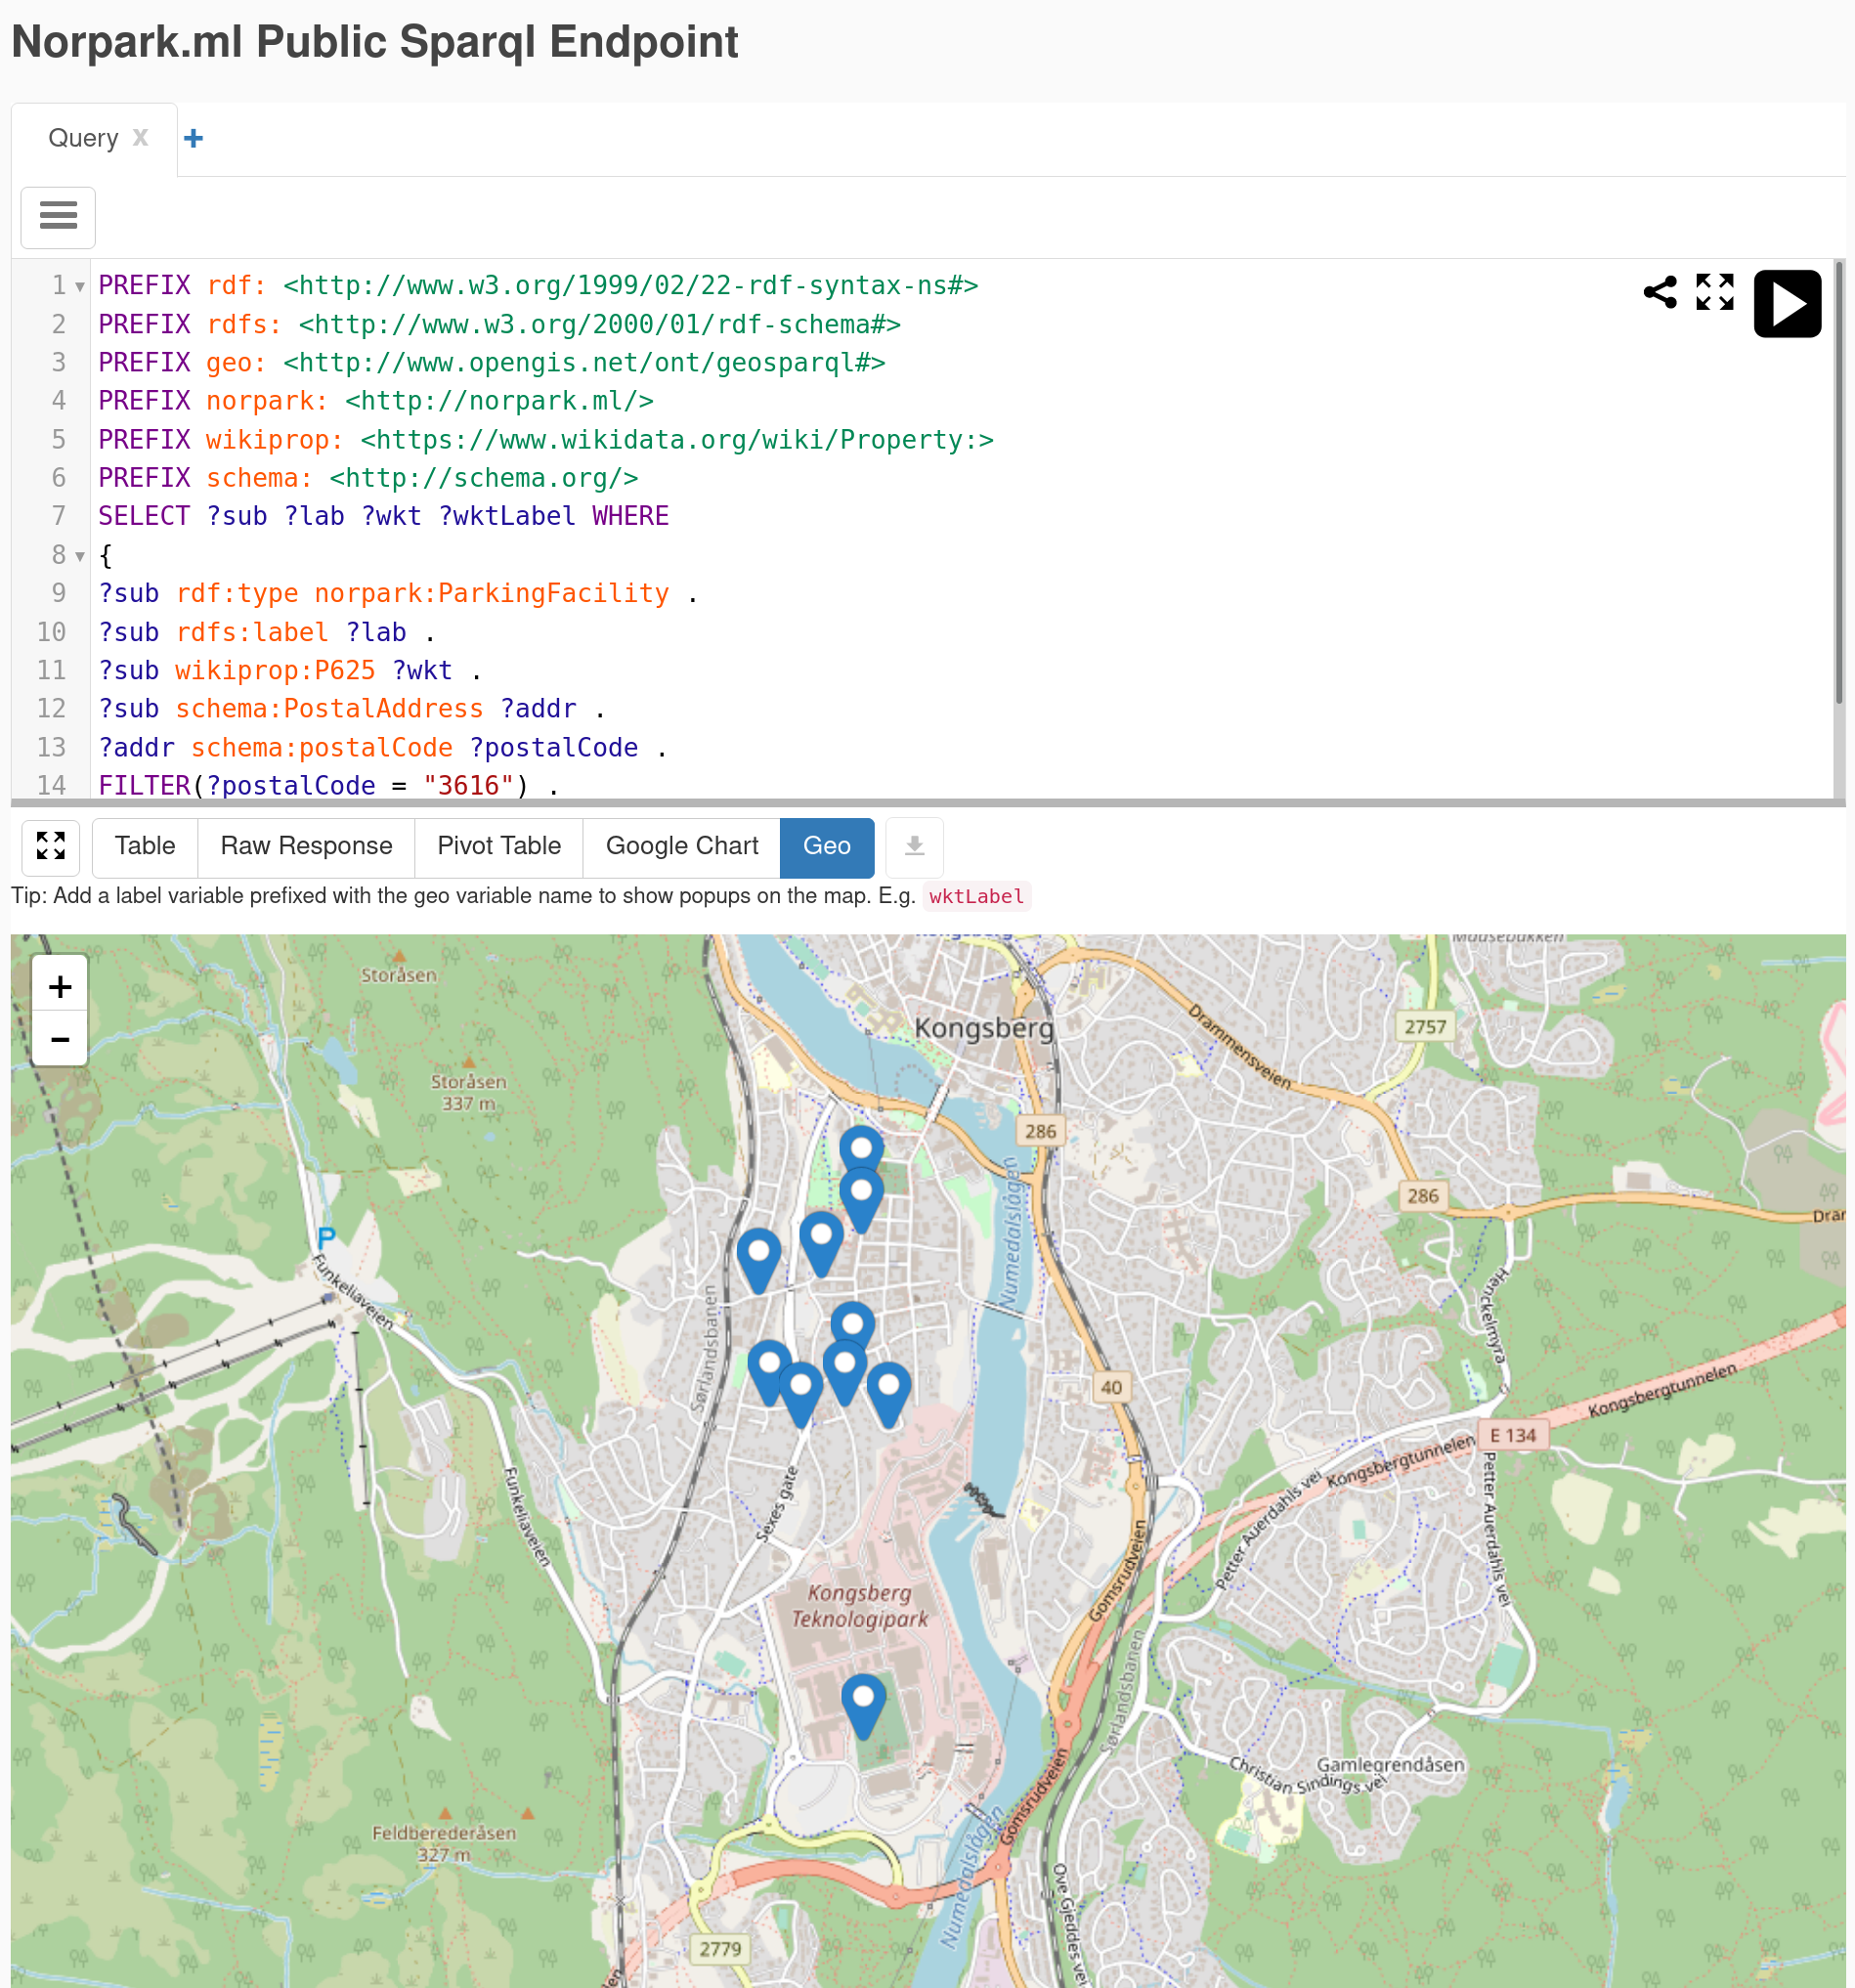
\includegraphics[width=\linewidth]{figures/query-screenshot.png}
	\caption{A screenshot LOD Cloud page for our dataset. }
\end{figure}

\chapter{Airflow workflow scheduler}
\label{appendix:airflow}
\begin{figure}[H]
	\centering
	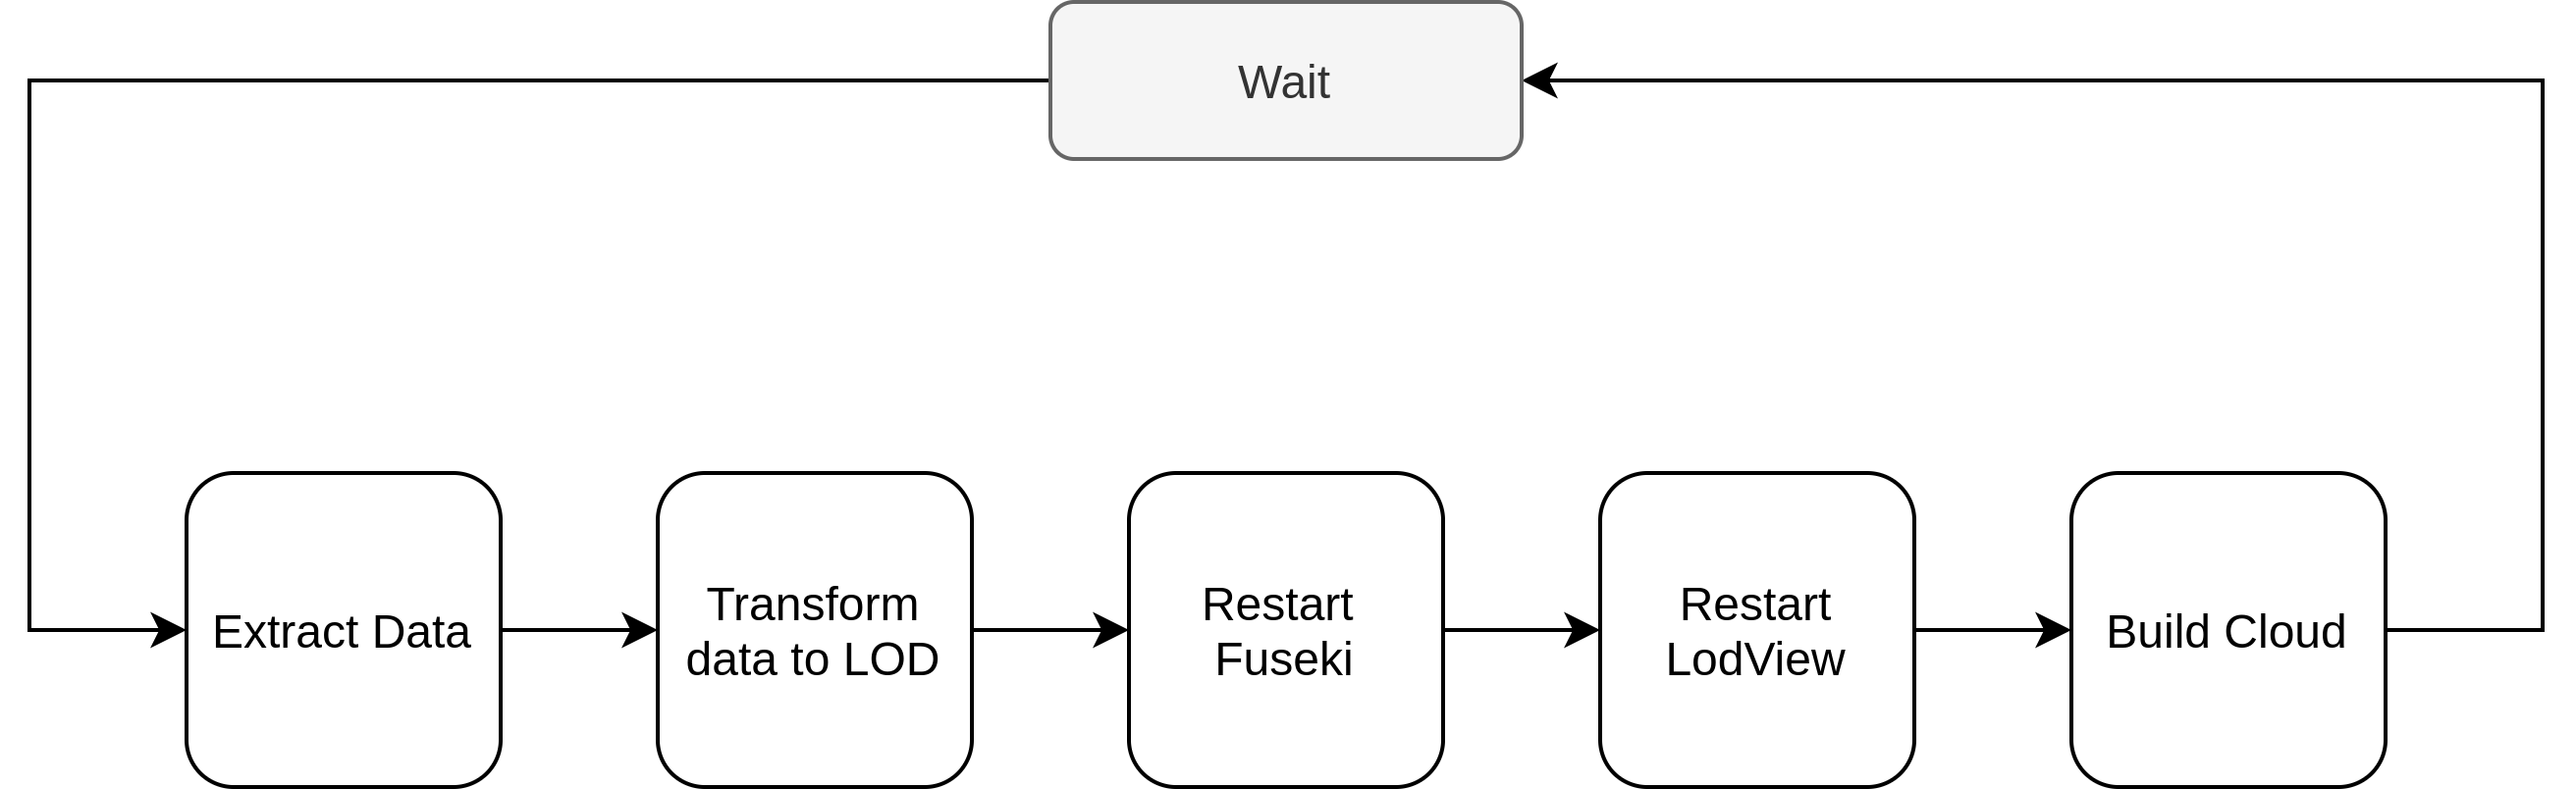
\includegraphics[width=\linewidth]{figures/airflow.png}
	\caption{A diagram of the Airflow workflow scheduler.}
\end{figure}

\end{document}
